\documentclass{article}
\usepackage{CJK}
\usepackage{tikz}
\usepackage{indentfirst}
\usepackage{amsmath}
\usepackage{amsfonts}
\usepackage{geometry}
\usepackage{graphicx}
\usepackage{epstopdf}
\usepackage{float}
\usepackage{arydshln}
\usetikzlibrary{graphs}
\geometry{a4paper,scale=0.8}
\begin{document}
\begin{CJK}{UTF8}{gbsn}
	\author{Canpei Hu}
	\title{Wavelet Review}
	\maketitle
\setlength{\parindent}{2em}


\section{向量空间、张成、基底}
	\textbf{向量空间}$\mathbb{V}$:
	\textcircled{1}对加法封闭:
		$\forall\boldsymbol{x},\boldsymbol{y}\in\mathbb{V}\Rightarrow \boldsymbol{x}+\boldsymbol{y}\in\mathbb{V}$
\\
	\indent\indent\indent\indent\textcircled{2}对数乘封闭:
		$\forall\boldsymbol{x}\in\mathbb{V},\forall\lambda\in\mathbb{R}\Rightarrow\lambda\boldsymbol{x}\in\mathbb{V}$\par
	\textbf{线性组合}:$\boldsymbol{z}=a\boldsymbol{x}+b\boldsymbol{y}\quad\boldsymbol{x},\boldsymbol{y},\boldsymbol{z}\in\mathbb{V};a,b\in\mathbb{R}$\par
	\textbf{张成}:$span\{\boldsymbol{v_1},\boldsymbol{v_2},\cdots,\boldsymbol{v_n}\}=
		\{a_1\boldsymbol{v_1}+a_2\boldsymbol{v_2}+\cdots+a_n\boldsymbol{v_n}|a_i\in\mathbb{R};\boldsymbol{v_i}\in\mathbb{V}\}$\par
	\textbf{基底}:空间中存在的最大线性无关向量组,即张成此空间所需的最小线性无关向量组\par
	$\mathbb{V}$的\textbf{子空间}:既是$\mathbb{V}$的子集,又是向量空间\\

\section{正交、相关、傅里叶级数的基底}
	同一空间中的两个\textbf{向量$\boldsymbol{x},\boldsymbol{y}$正交},即是$\boldsymbol{x^T}\boldsymbol{y}=\boldsymbol{x}\cdot\boldsymbol{y}=0$;\par
	$[a,b]$区间上的两个\textbf{函数$f(x),g(x)$正交},即是$\int_a^bf(x)g(x)dx=0$.\par
	以上定义引入\textbf{内积}概念:向量$\boldsymbol{x},\boldsymbol{y}$的内积定义为$\sum_{i=1}^nx_iy_i$;$[a,b]$区间上函数$f(x),g(x)$的内积定义为$\int_a^bf(x)g(x)dx$.\par
	\textbf{相关}亦由内积定义,内积的模越大,相关性越强。正交即是相关为0的特殊情况。\par
	三角函数系$\{1,cosx,sinx,cos2x,sin2x,\cdots,cosnx,sinnx\}$在基波$\{cosx,sinx\}$的周期区间上正交,且每一个基底与自身内积为1,
	它们是傅里叶级数空间的一组\textbf{标准正交基(orthonormal basis)}.\\
	基底选择三原则:\par
	\textbf{\textcircled{1}正交(orthogonal)}:一组基底中的向量两两正交,实现计算时的\textbf{解耦(decouple)},
	并且最好是\textbf{归一化(normalized)}的,称为\textbf{标准正交基(orthonormal basis)};\par
	\textbf{\textcircled{2}系数紧凑(compact coefficients)}:向量在少量基底上的投影系数大,而在绝大部分基底上的投影系数小;\par
	\textbf{\textcircled{3}特征包含}:含有一个向量想要测量的性质。\\

\section{矩阵4个子空间、正交补}
	$\boldsymbol{A}$的\textbf{列空间}$\mathbb{C}(\boldsymbol{A})$:
	$\boldsymbol{A}$的列向量张成的空间\par
	$\boldsymbol{A}$的\textbf{零空间}$\mathbb{N}(\boldsymbol{A})$:
	方程$\boldsymbol{Ax}=0$的解空间\par
	$\boldsymbol{A}^T$的列空间$\mathbb{C}(\boldsymbol{A}^T)$:
	$\boldsymbol{A}^T$的列向量张成的空间\par
	$\boldsymbol{A}^T$的零空间$\mathbb{N}(\boldsymbol{A}^T)$:
	方程$\boldsymbol{A}^T\boldsymbol{x}=0$的解空间\par
	$\mathbb{V}_0$在$\mathbb{V}$中的\textbf{正交补}:$\{\boldsymbol{v}\in\mathbb{V}|\forall\boldsymbol{v_0}\in\mathbb{V}_0\Rightarrow\boldsymbol{v}\cdot\boldsymbol{v_0}=0\}$.
	子空间的正交补也是子空间。\\
	关系:\\
	\textcircled{1}$\boldsymbol{A}^T$的列空间是$\boldsymbol{A}$的\textbf{行空间},即$\boldsymbol{A}$的行向量张成的空间\\
	\textcircled{2}$\boldsymbol{A}^T$的零空间是$\boldsymbol{A}$的\textbf{左零空间},即方程$\boldsymbol{xA}=0$的解空间\\
	\textcircled{3}$\mathbb{C}(\boldsymbol{A}) \perp \mathbb{N}(\boldsymbol{A}^T)$,二者互为正交补
	,即$\forall\boldsymbol{x}\in\mathbb{C}(\boldsymbol{A}),\forall\boldsymbol{y}\in\mathbb{N}(\boldsymbol{A}^T)\Rightarrow\boldsymbol{x}\cdot\boldsymbol{y}=0$\\
	\textcircled{4}$\mathbb{C}(\boldsymbol{A}^T) \perp \mathbb{N}(\boldsymbol{A})$,二者互为正交补
	,即$\forall\boldsymbol{x}\in\mathbb{C}(\boldsymbol{A}^T),\forall\boldsymbol{y}\in\mathbb{N}(\boldsymbol{A})\Rightarrow\boldsymbol{x}\cdot\boldsymbol{y}=0$\\

		
\section{一个向量用另一个向量近似}
\begin{figure}[H]
\centering  
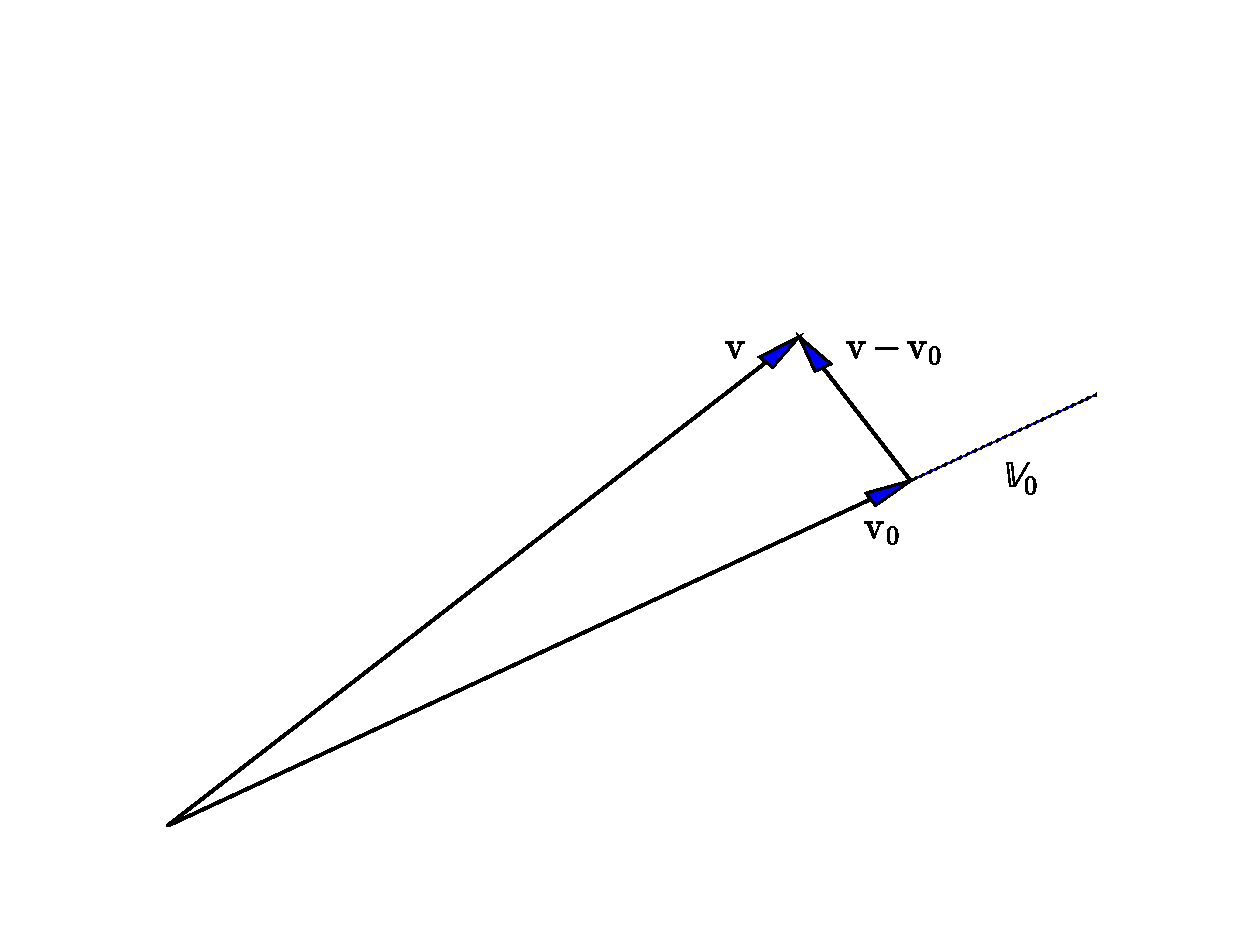
\includegraphics[height=7cm,width=9cm]{./figs/fig1.eps}  
\caption{一个向量用另一个向量近似}
\label{1}  
\end{figure}
	如图Fig1,用子空间$\mathbb{V}_0$中的$\alpha\boldsymbol{v_0}$来近似表达$\mathbb{V}$中的向量$\boldsymbol{v}$.
	要使得误差$\boldsymbol{v}-\alpha\boldsymbol{v_0}$最小,
	即是求$$\boldsymbol{J}=\parallel\boldsymbol{v}-\alpha\boldsymbol{v_0}\parallel ^2$$最小时的$\alpha$,可用如下方法:\par
	\indent\textcircled{1}J对$\alpha$求导;\par
	\indent\textcircled{2}用垂线最短:
	$$(\boldsymbol{v}-\alpha\boldsymbol{v_0})\perp\boldsymbol{v_0} 
	\Rightarrow
	(\boldsymbol{v}-\alpha\boldsymbol{v_0})\cdot\boldsymbol{v_0}=0
	\Rightarrow
	\alpha =\frac{\boldsymbol{v}\cdot\boldsymbol{v_0}}{\boldsymbol{v_0}\cdot\boldsymbol{v_0}}$$\\


\section{一个向量用另一组向量近似、正交投影}
\begin{figure}[H]
\centering
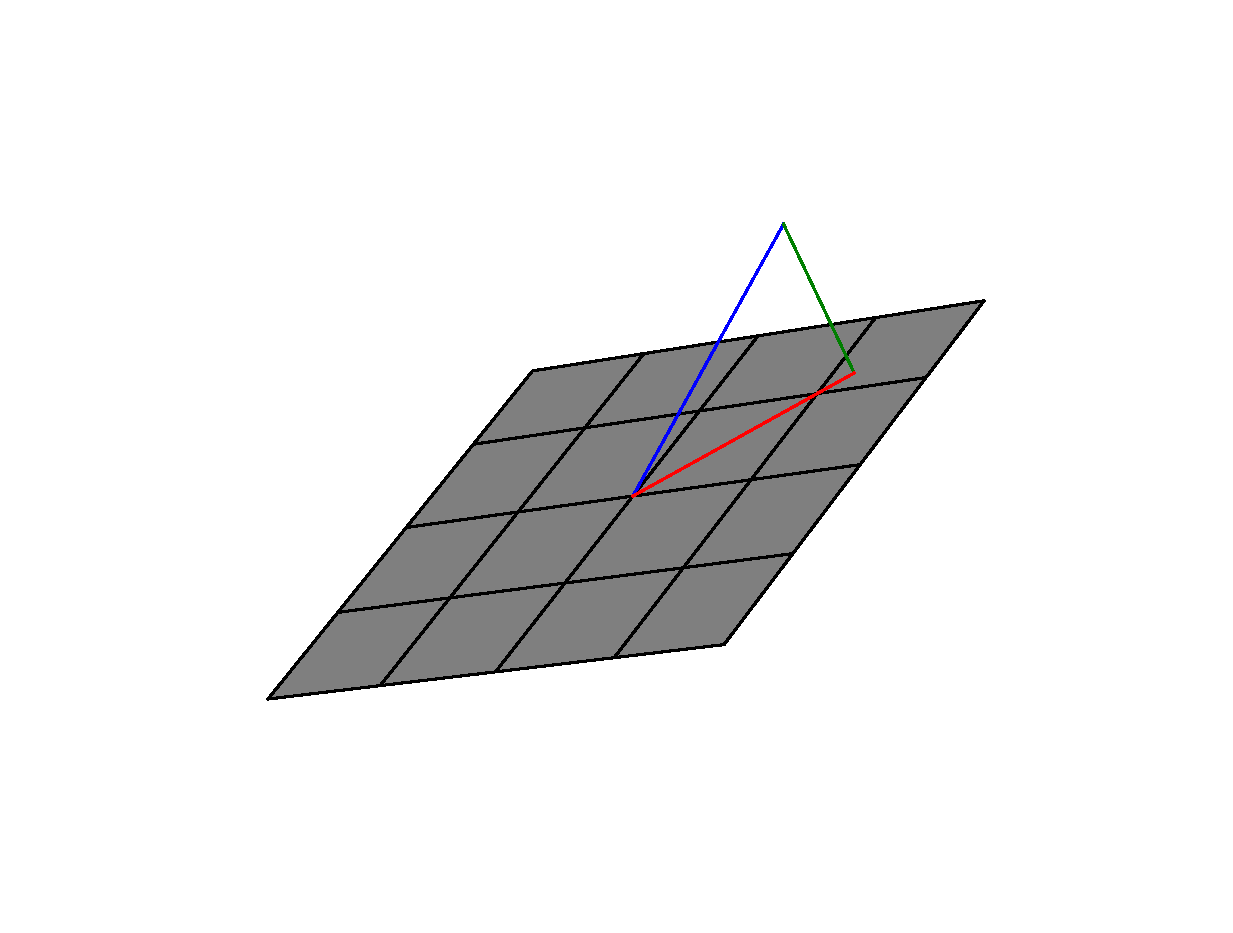
\includegraphics[height=7cm,width=9cm]{./figs/fig2.eps}
\caption{一个向量用另一组向量近似}
\label{2}
\end{figure}
	引入\textbf{正交投影}:若$\mathbb{V}_0$是$\mathbb{V}$的子空间,则$\mathbb{V}$中向量$\boldsymbol{v}$在$\mathbb{V}_0$中的正交投影$\boldsymbol{v_0}$满足:
	\textcircled{1}$\boldsymbol{v_0}\in\mathbb{V}_0$;\textcircled{2}$\boldsymbol{v}-\boldsymbol{v_0}$与$\mathbb{V}_0$中所有向量都正交。\par
	若$\boldsymbol{v}\in\mathbb{V}_0$,则$\boldsymbol{v}$的正交投影就是它本身;
	若$\boldsymbol{v}\notin\mathbb{V}_0$,则$\boldsymbol{v}-\boldsymbol{v_0}$垂直于$\mathbb{V}_0$的所有基底。\par
	将前文中一个向量近似的情形推广到一组向量,以两个为例。\par
	如图,用子空间$\mathbb{V}_0$的基底$\boldsymbol{v_1},\boldsymbol{v_2}$来近似表达$\mathbb{V}$中的向量$\boldsymbol{v}$,
	使得误差$\boldsymbol{v}-\alpha\boldsymbol{v_1}-\beta\boldsymbol{v_2}$最小,
	即是求$$\boldsymbol{J}=\parallel\boldsymbol{v}-(\alpha\boldsymbol{v_1}+\beta\boldsymbol{v_2})\parallel ^2$$最小时的$\alpha,\beta$.\\
	\indent\textcircled{1}用高数方法求取到极值时的条件;\\
    \indent\textcircled{2}用正交投影:
	$$(\boldsymbol{v}-\alpha\boldsymbol{v_1}-\beta\boldsymbol{v_2})\perp\mathbb{V}_0
	\Rightarrow\left\{\begin{aligned}(\boldsymbol{v}-\alpha\boldsymbol{v_1}-\beta\boldsymbol{v_2})\perp\boldsymbol{v_1}\\
	(\boldsymbol{v}-\alpha\boldsymbol{v_1}-\beta\boldsymbol{v_2})\perp\boldsymbol{v_2}\end{aligned}\right.
	\Rightarrow\left\{\begin{aligned}\boldsymbol{v}\cdot\boldsymbol{v_1}=\alpha\boldsymbol{v_1}\cdot\boldsymbol{v_1}+\beta\boldsymbol{v_2}\cdot\boldsymbol{v_1}\\
	\boldsymbol{v}\cdot\boldsymbol{v_2}=\alpha\boldsymbol{v_1}\cdot\boldsymbol{v_2}+\beta\boldsymbol{v_2}\cdot\boldsymbol{v_2}\end{aligned}\right.$$\\
	二元一次,解出$\alpha,\beta$即可。\\


\section{最小二乘}
	最小二乘的求解思路即是用一组向量近似一个向量。
	考虑含有两个特征的方程组:
	$$\left\{\begin{aligned}m_1x^1_1+n_1x^2_1+b_1=y_1\\m_2x^1_2+n_2x^2_2+b_2=y_2\\ \cdots\\m_kx^1_k+n_kx^2_k+b_k=y_k\end{aligned}\right.$$
	写为向量形式$\boldsymbol{m}\cdot\boldsymbol{x^1}+\boldsymbol{n}\cdot\boldsymbol{x^2}+\boldsymbol{b}\cdot\boldsymbol{u}=\boldsymbol{y}$.\par
	一般来说,这个方程组的变量维度远远高于特征数,不存在确切解。因此最小二乘的目的即是找一个方程,它能由这一组方程表示,使得表示误差最小。
	这等价于找一点$\boldsymbol{p}=m\boldsymbol{x^1}+n\boldsymbol{x^2}+b\boldsymbol{u}$,使得$\boldsymbol{p}$与$\boldsymbol{y}$误差最小。\par
	由前文向量近似表达的思想,做如下推导:
	$$\left\{\begin{aligned}(\boldsymbol{y}-\boldsymbol{p})&\perp&\boldsymbol{x^1}\\
	(\boldsymbol{y}-\boldsymbol{p})&\perp&\boldsymbol{x^2}\\
	(\boldsymbol{y}-\boldsymbol{p})&\perp&\boldsymbol{u}\end{aligned}\right.
	\Rightarrow
	\left\{\begin{aligned}(\boldsymbol{y}-m\boldsymbol{x^1}-n\boldsymbol{x^2}-b\boldsymbol{u})\cdot\boldsymbol{x^1} &=& 0\\
	(\boldsymbol{y}-m\boldsymbol{x^1}-n\boldsymbol{x^2}-b\boldsymbol{u})\cdot\boldsymbol{x^2} &=& 0\\
	(\boldsymbol{y}-m\boldsymbol{x^1}-n\boldsymbol{x^2}-b\boldsymbol{u})\cdot\boldsymbol{u} &=& 0\end{aligned}\right.
	\Rightarrow
	\left\{\begin{aligned}\boldsymbol{x^1}\cdot\boldsymbol{y} &=& m\boldsymbol{x^1}\cdot\boldsymbol{x^1}+n\boldsymbol{x^2}\cdot\boldsymbol{x^1}+b\boldsymbol{u}\cdot\boldsymbol{x^1}\\
	\boldsymbol{x^2}\cdot\boldsymbol{y} &=& m\boldsymbol{x^1}\cdot\boldsymbol{x^2}+n\boldsymbol{x^2}\cdot\boldsymbol{x^2}+b\boldsymbol{u}\cdot\boldsymbol{x^2}\\
	\boldsymbol{u}\cdot\boldsymbol{y} &=& m\boldsymbol{x^1}\cdot\boldsymbol{u}+n\boldsymbol{x^2}\cdot\boldsymbol{u}+b\boldsymbol{u}\cdot\boldsymbol{u}\end{aligned}\right.$$
	写为矩阵形式:
	$$\left\{\begin{aligned}\boldsymbol{x^{1T}}\boldsymbol{y} &=& m\boldsymbol{x^{1T}}\boldsymbol{x^1}+n\boldsymbol{x^{2T}}\boldsymbol{x^1}+b\boldsymbol{u^T}\boldsymbol{x^1}\\
	\boldsymbol{x^{2T}}\boldsymbol{y} &=& m\boldsymbol{x^{1T}}\boldsymbol{x^2}+n\boldsymbol{x^{2T}}\boldsymbol{x^2}+b\boldsymbol{u^T}\boldsymbol{x^2}\\
	\boldsymbol{u^T}\boldsymbol{y} &=& m\boldsymbol{x^{1T}}\boldsymbol{u}+n\boldsymbol{x^{2T}}\boldsymbol{u}+b\boldsymbol{u^T}\boldsymbol{u}\end{aligned}\right.
	\Rightarrow
	\left [\begin{array}{cccc}\boldsymbol{x^{1T}}\\\boldsymbol{x^{2T}}\\\boldsymbol{u^T}\end{array}\right ]\boldsymbol{y}=
	\left [\begin{array}{cccc}\boldsymbol{x^{1T}}\\\boldsymbol{x^{2T}}\\\boldsymbol{u^T}\end{array}\right ]
	\left [\begin{array}{cccc}\boldsymbol{x^1}&\boldsymbol{x^2}&\boldsymbol{u}\end{array}\right ]
	\left [\begin{array}{cccc}m\\n\\b\end{array}\right ]$$
	令$\boldsymbol{Z}=\left [\begin{array}{cccc}\boldsymbol{x^1}&\boldsymbol{x^2}&\boldsymbol{u}\end{array}\right ]$,则有:
	$\left [\begin{array}{cccc}m\\n\\b\end{array}\right ]=(\boldsymbol{Z^T}\boldsymbol{Z})^{-1}\boldsymbol{Z^T}\boldsymbol{y}$\\
	这就是\textbf{最小二乘法(Least Square Method,LSM)}。\\

	
\section{Haar小波的三种理解}
\begin{figure}[H]
\centering
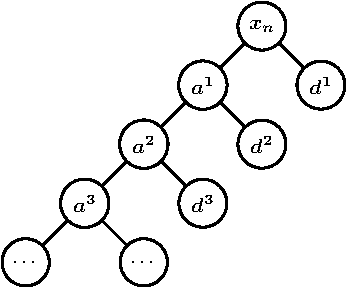
\includegraphics[height=5cm,width=6cm]{./figs/fig3.pdf}
\caption{Haar小波分解}
\label{3}
\end{figure}
	Fig3为小波每一层的分解图,不断分解$\boldsymbol{a}$分量即可。\\
	\textbf{\textcircled{1}:运算观点}\par
	给定序列(向量)$\boldsymbol{x_n}=\{x_1,x_2,\cdots,x_N\}$,其中$N=2^m$是2的整数幂。
	则$\boldsymbol{x_n}$的一级Haar小波分解如下:
	$$\boldsymbol{a^1}=\{\frac{x_1+x_2}{\sqrt{2}},\frac{x_3+x_4}{\sqrt{2}},\cdots,\frac{x_{N-1}+x_N}{\sqrt{2}}\}$$
	$$\boldsymbol{d^1}=\{\frac{x_1-x_2}{\sqrt{2}},\frac{x_3-x_4}{\sqrt{2}},\cdots,\frac{x_{N-1}-x_N}{\sqrt{2}}\}$$
	注意其中$\boldsymbol{a^1}$和$\boldsymbol{d^1}$的长度(维度)为$\frac{N}{2}$。
	对$\boldsymbol{a^1}$继续应用如上变换,得到
	$$\boldsymbol{a^2}=\{\frac{a^1_1+a^1_2}{\sqrt{2}},\frac{a^1_3+a^1_4}{\sqrt{2}},\cdots,\frac{a^1_{\frac{N}{2}-1}+a^1_{\frac{N}{2}}}{\sqrt{2}}\}=\{\frac{x_1+x_2+x_3+x_4}{2},\frac{x_5+x_6+x_7+x_8}{2},\cdots\}$$
    $$\boldsymbol{d^2}=\{\frac{a^1_1-a^1_2}{\sqrt{2}},\frac{a^1_3-a^1_4}{\sqrt{2}},\cdots,\frac{a^1_{\frac{N}{2}-1}-a^1_{\frac{N}{2}}}{\sqrt{2}}\}=\{\frac{x_1+x_2-x_3-x_4}{2},\frac{x_5+x_6-x_7-x_8}{2},\cdots\}$$
	注意其中$\boldsymbol{a^2}$和$\boldsymbol{d^2}$的维度为$\frac{N}{4}$,此即为$\boldsymbol{x_n}$的二级Haar小波分解\par
	更高阶的小波分解依此类推,不断对$\boldsymbol{a^i}$分解,每次维度减半。\\
	\textbf{\textcircled{2}:基底观点}\par
	定义N维向量空间$\mathbb{U}^1,\mathbb{V}^1,\mathbb{U}^2,\mathbb{V}^2,\cdots$,其中$\mathbb{U}^1$的基底为:
	$$\boldsymbol{u^1_1}=[\frac{1}{\sqrt{2}},\frac{1}{\sqrt{2}},0,0,0,0,\cdots]^T$$
	$$\boldsymbol{u^1_2}=[0,0,\frac{1}{\sqrt{2}},\frac{1}{\sqrt{2}},0,0,\cdots]^T$$
	$$\cdots$$
	$$\boldsymbol{u^1_{\frac{N}{2}}}=[0,0,\cdots,0,0,\frac{1}{\sqrt{2}},\frac{1}{\sqrt{2}}]^T$$
	$\mathbb{V}^1$的基底为:
	$$\boldsymbol{v^1_1}=[\frac{1}{\sqrt{2}},-\frac{1}{\sqrt{2}},0,0,0,0,\cdots]^T$$
    $$\boldsymbol{v^1_2}=[0,0,\frac{1}{\sqrt{2}},-\frac{1}{\sqrt{2}},0,0,\cdots]^T$$
    $$\cdots$$
    $$\boldsymbol{v^1_{\frac{N}{2}}}=[0,0,\cdots,0,0,\frac{1}{\sqrt{2}},-\frac{1}{\sqrt{2}}]^T$$
	$\mathbb{U}^2$的基底为:
    $$\boldsymbol{u^2_1}=[\frac{1}{\sqrt{4}},\frac{1}{\sqrt{4}},\frac{1}{\sqrt{4}},\frac{1}{\sqrt{4}},0,0,0,0,0,0,0,0,\cdots]^T$$
    $$\boldsymbol{u^2_2}=[0,0,0,0,\frac{1}{\sqrt{4}},\frac{1}{\sqrt{4}},\frac{1}{\sqrt{4}},\frac{1}{\sqrt{4}},0,0,0,0,\cdots]^T$$
    $$\cdots$$
    $$\boldsymbol{u^2_{\frac{N}{4}}}=[0,0,0,0,\cdots,0,0,0,0,\frac{1}{\sqrt{4}},\frac{1}{\sqrt{4}},\frac{1}{\sqrt{4}},\frac{1}{\sqrt{4}}]^T$$
	$\mathbb{V}^2$的基底为:
    $$\boldsymbol{v^2_1}=[\frac{1}{\sqrt{4}},\frac{1}{\sqrt{4}},-\frac{1}{\sqrt{4}},-\frac{1}{\sqrt{4}},0,0,0,0,0,0,0,0,\cdots]^T$$
    $$\boldsymbol{v^2_2}=[0,0,0,0,\frac{1}{\sqrt{4}},\frac{1}{\sqrt{4}},-\frac{1}{\sqrt{4}},-\frac{1}{\sqrt{4}},0,0,0,0,\cdots]^T$$
    $$\cdots$$
    $$\boldsymbol{v^2_{\frac{N}{4}}}=[0,0,0,0,\cdots,0,0,0,0,\frac{1}{\sqrt{4}},\frac{1}{\sqrt{4}},-\frac{1}{\sqrt{4}},-\frac{1}{\sqrt{4}}]^T$$
	更高阶依此类推,每个基底的\textbf{支撑(support)}数量按2的指数递增,空间的基底数量按2的指数递减。注意这些向量都是N维的。\par
	$\mathbb{U}^1,\mathbb{V}^1$是一对正交补,所有向量$\{\boldsymbol{u^1_i},\boldsymbol{v^1_i}\}$构成$\mathbb{R}^N$的一组单位正交基。
	同理,$\mathbb{U}^2,\mathbb{V}^2$是一对正交补,所有向量$\{\boldsymbol{u^2_i},\boldsymbol{v^2_i}\}$构成$span\{\boldsymbol{u^1_i}\}$的一组单位正交基。
	在这个基础上,构建\textbf{尺度分量}$\boldsymbol{a}$和\textbf{小波分量}$\boldsymbol{d}$
	$$\boldsymbol{a^1}=\begin{bmatrix}\boldsymbol{x}\cdot\boldsymbol{u^1_1}&\boldsymbol{x}\cdot\boldsymbol{u^1_2}&\cdots&\boldsymbol{x}\cdot\boldsymbol{u^1_{\frac{N}{2}}}\end{bmatrix}^T$$
	$$\boldsymbol{d^1}=\begin{bmatrix}\boldsymbol{x}\cdot\boldsymbol{v^1_1}&\boldsymbol{x}\cdot\boldsymbol{v^1_2}&\cdots&\boldsymbol{x}\cdot\boldsymbol{v^1_{\frac{N}{2}}}\end{bmatrix}^T$$
	$$\boldsymbol{a^2}=\begin{bmatrix}\boldsymbol{x}\cdot\boldsymbol{u^2_1}&\boldsymbol{x}\cdot\boldsymbol{u^2_2}&\cdots&\boldsymbol{x}\cdot\boldsymbol{u^2_{\frac{N}{4}}}\end{bmatrix}^T$$
	$$\boldsymbol{d^2}=\begin{bmatrix}\boldsymbol{x}\cdot\boldsymbol{v^2_1}&\boldsymbol{x}\cdot\boldsymbol{v^2_2}&\cdots&\boldsymbol{x}\cdot\boldsymbol{v^2_{\frac{N}{4}}}\end{bmatrix}^T$$
	这样,就在向量空间的基础上理解了小波分解。\\	
	\textbf{\textcircled{3}:图像观点}\par
	将序列下标改为连续变量,作图如下:
\begin{figure}[H]
\centering
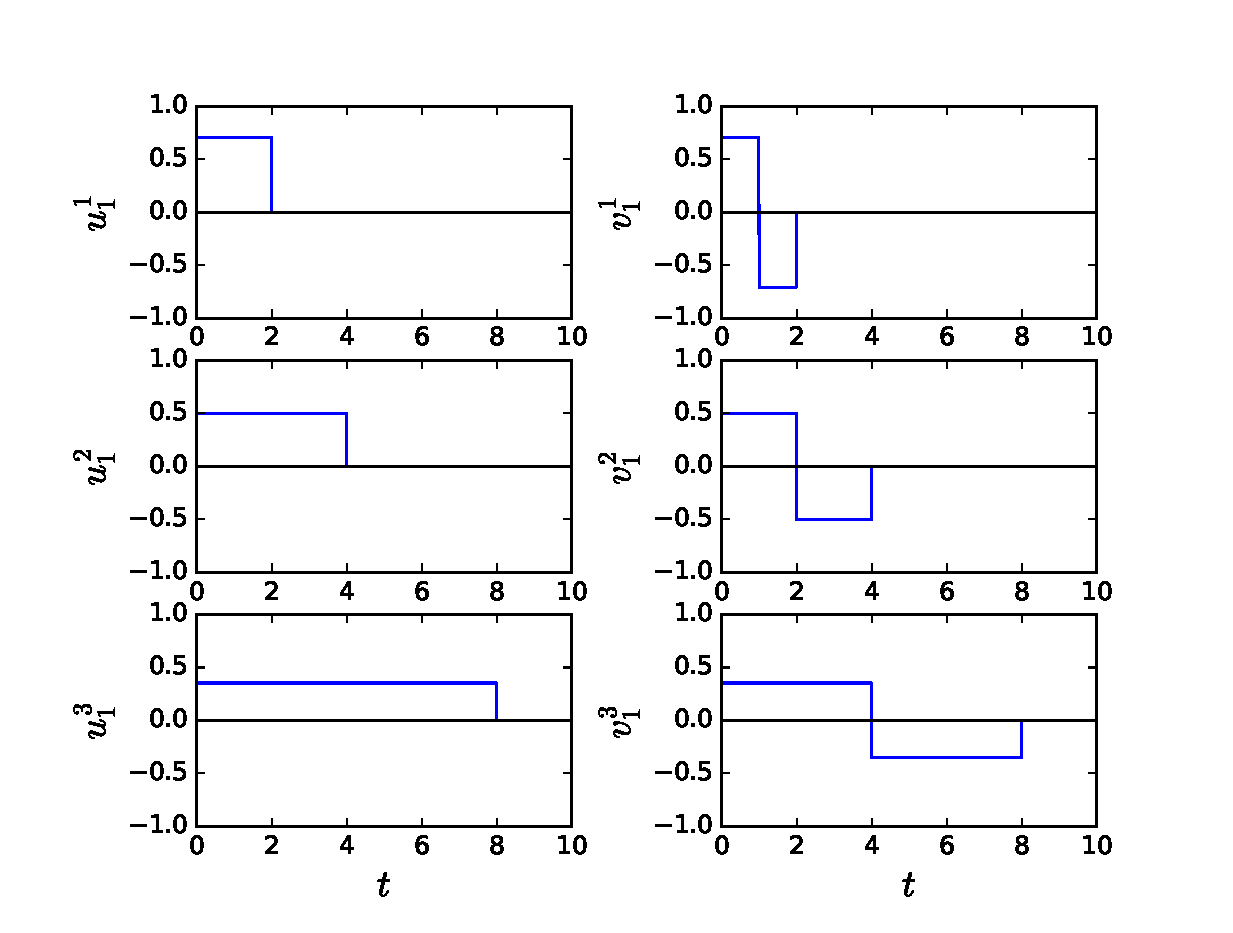
\includegraphics[height=8cm,width=12cm]{./figs/fig4.eps}
\caption{Haar小波基}
\label{4}
\end{figure}
	从前文可以看出,$\boldsymbol{u^1_1}$向右平移2得到$\boldsymbol{u^1_2}$,$\boldsymbol{u^1_1}$向右平移4得到$\boldsymbol{u^1_3}$;
	$\boldsymbol{u^2_1}$向右平移4得到$\boldsymbol{u^2_2}$,$\boldsymbol{u^2_1}$向右平移8得到$\boldsymbol{u^2_3}$,其余规律以此类推。\par
	上面连续形式的$\boldsymbol{u^i_j},\boldsymbol{v^i_j}$构成一组小波基,对于任何均方收敛的函数,都可以表示为若干小波基的线性组合,即若干小波基波形的叠加。\\
	

\section{二维Haar小波基}
	前面已经引入连续形式的一级小波基,这里介绍尺度函数和小波函数,仅讨论一级分解(实际上二级分解即是取一级分解得到的尺度分量继续分解)。\par
	\textbf{尺度函数(父小波)}即是前文中的$\boldsymbol{u^i_j}$,用来描述小波变换的尺度,连续情形下记作函数$\phi(x)$\par
	\textbf{小波函数(母小波)}即是前文中的$\boldsymbol{v^i_j}$,用来描述该尺度下的小波变换,连续情形下记作函数$\psi(x)$\par
	二维情形下,只有两个一维尺度函数相乘才能得到二维尺度函数,即$$\phi(x,y)=\phi(x)\phi(y)$$
	而其他三种乘积均得到不同方向上的二维小波函数$$\psi^1(x,y)=\phi(x)\psi(y),\quad\psi^2(x,y)=\psi(x)\phi(y),\quad\psi^3(x,y)=\psi(x)\psi(y)$$
	将其写为离散形式并忽略所有零元素(实际上得到的矩阵是稀疏的,这里我只取非零元):\\
	\textbf{尺度函数}(水平父、垂直父)(LL):
	$$\phi(x,y)=\phi(x)\phi(y)=\begin{bmatrix}\frac{1}{\sqrt{2}}\\\frac{1}{\sqrt{2}}\end{bmatrix}\begin{bmatrix}\frac{1}{\sqrt{2}}&\frac{1}{\sqrt{2}}\end{bmatrix}=\begin{bmatrix}\frac{1}{2}&\frac{1}{2}\\\frac{1}{2}&\frac{1}{2}\end{bmatrix}$$\\
	\textbf{水平小波函数}(水平母、垂直父)(HL):
	$$\psi^1(x,y)=\phi(x)\psi(y)=\begin{bmatrix}\frac{1}{\sqrt{2}}\\\frac{1}{\sqrt{2}}\end{bmatrix}\begin{bmatrix}\frac{1}{\sqrt{2}}&-\frac{1}{\sqrt{2}}\end{bmatrix}=\begin{bmatrix}\frac{1}{2}&-\frac{1}{2}\\\frac{1}{2}&-\frac{1}{2}\end{bmatrix}$$\\
	\textbf{垂直小波函数}(水平父、垂直母)(LH):
	$$\psi^2(x,y)=\psi(x)\phi(y)=\begin{bmatrix}\frac{1}{\sqrt{2}}\\-\frac{1}{\sqrt{2}}\end{bmatrix}\begin{bmatrix}\frac{1}{\sqrt{2}}&\frac{1}{\sqrt{2}}\end{bmatrix}=\begin{bmatrix}\frac{1}{2}&\frac{1}{2}\\-\frac{1}{2}&-\frac{1}{2}\end{bmatrix}$$\\
	\textbf{对角小波函数}(水平母、垂直母)(HH):
	$$\psi^3(x,y)=\psi(x)\psi(y)=\begin{bmatrix}\frac{1}{\sqrt{2}}\\-\frac{1}{\sqrt{2}}\end{bmatrix}\begin{bmatrix}\frac{1}{\sqrt{2}}&-\frac{1}{\sqrt{2}}\end{bmatrix}=\begin{bmatrix}\frac{1}{2}&-\frac{1}{2}\\-\frac{1}{2}&\frac{1}{2}\end{bmatrix}$$\par
	一般来说,对图像(矩阵)做Haar分解:LL保留原图像的主要内容,HL保留水平方向的高频信息,LH保留竖直方向的高频信息,HH保持对角线方向的高频信息。\\

\section{FT、STFT、WT的关系}
\begin{figure}[H]
\centering
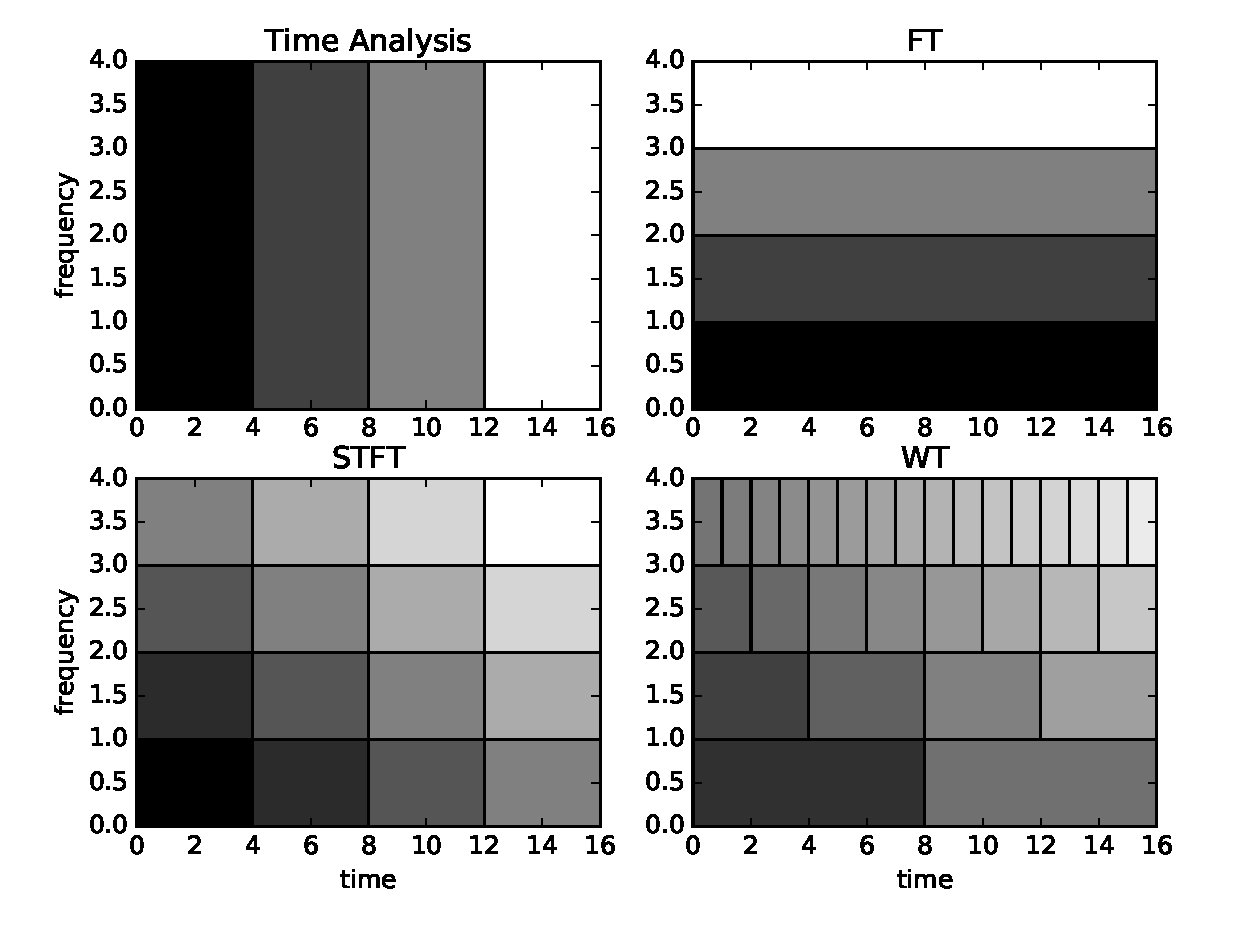
\includegraphics[height=7cm,width=9cm]{./figs/fig5.eps}
\caption{FT,STFT,WT的关系}
\label{5}
\end{figure}
	在\textbf{时域分析(Time Analysis)}中无法得到频域信息,而\textbf{傅里叶变换(Fourier Transform)}无法得到时域信息(如图中上面两幅图,左图只具备时间分辨率,右图只具备频率分辨率)。
	基于这两种方法的局限性,后来提出了\textbf{短时傅里叶变换(Short-Time Fourier Transform)}和\textbf{小波变换(Wavelet Transform)}.\par
	STFT是将时间轴分段,每一段上分别进行FT,这样做得到的时频域分辨率如左下图。然而由时间和频率的不确定性原理,更低的频率需要更长的时间块来描述,而一旦时间块变长,对于较高频率而言STFT的意义也就不存在。这就产生了一对矛盾。\par
	WT也是将时间轴分段,但与STFT不同的是,WT是非均匀分段,在较高频率处使用小的时间块刻画,在较低频率处使用大的时间块刻画,进行了一定程度上的折中。这一良好性质的理论基础是各级小波分解中的尺度函数。\par
	不过需注意小波仍然没有克服时间和频率的不确定性,克服这一不确定性的变换有\textbf{希尔伯特-黄变换(HHT)}等。\\


\section{WT的应用}
	\textcircled{1}图像去噪、压缩(指纹图片压缩、JPEG2000编码):舍弃高频成分,保留尺度分量。压缩比高,速度快,信息丢失少,传输过程抗干扰;\par
	\textcircled{2}数值计算:存在快速变换方法(滤波器组实现),对N点序列的时间复杂度为$\boldsymbol{O}(N)$,可用于计算傅里叶变换等;\par
	\textcircled{3}多分辨率处理、压缩感知;\par
	\textcircled{4}信号的时频分析;\par
	\textcircled{5}$\cdots\cdots$\\

\section{SVD分解、PCA}
	回顾\textbf{特征值分解(Eigen Value Decompostion,EVD)}:若对于矩阵$\boldsymbol{A}$和向量$\boldsymbol{x}$、标量$\lambda$,
	有$\boldsymbol{A}\boldsymbol{x}=\lambda\boldsymbol{x}$,
	则称$\boldsymbol{x}$为$\boldsymbol{A}$的特征向量,$\lambda$为$\boldsymbol{A}$的特征值(Eigen Value).
	特征向量的含义是,该向量$\boldsymbol{x}$在该变换$\boldsymbol{A}$下的结果方向不变,尺度变为原来的$\lambda$倍。\par
	将特征向量排成一个矩阵的列,记作$\boldsymbol{P}$;将相应的特征值写为对角阵,记作$\boldsymbol{\Lambda}$,则有$\boldsymbol{A}=\boldsymbol{P}\boldsymbol{\Lambda}\boldsymbol{P^{-1}}$.
	对于实对称阵$\boldsymbol{A}$,所有特征向量组成一组正交基,即排成正交阵$\boldsymbol{P}$,
	使得$\boldsymbol{A}=\boldsymbol{P}\boldsymbol{\Lambda}\boldsymbol{P^{-1}}=\boldsymbol{P}\boldsymbol{\Lambda}\boldsymbol{P^{T}}$.\par
	但是EVD的局限性在于,只有方阵才能做EVD,而实际使用的矩阵(如最小二乘的系数矩阵)往往不是方阵。因此提出问题:
	对任意的$m\times n$矩阵$\boldsymbol{A_{m\times n}}$,能否找到n维空间中的一组正交基,使其经过$\boldsymbol{A}$变换后,成为m维空间中的一组正交基?\par
	对任意$m\times n$矩阵$\boldsymbol{A_{m\times n}}$,$\boldsymbol{A^T}\boldsymbol{A}$是$n\times n$实对称阵,
	因而其特征向量是n维空间的一组正交基,记为$\{\boldsymbol{v_1},\boldsymbol{v_2},\cdots,\boldsymbol{v_n}\}$,
	则$\boldsymbol{A}$将其映射为$\{\boldsymbol{Av_1},\boldsymbol{Av_2},\cdots,\boldsymbol{Av_n}\}$。	
	由于$\{\boldsymbol{v}\}$本身正交,有$\boldsymbol{v^T_iv_j}=0$,
	且$$\boldsymbol{(Av_i)^TAv_j}=\boldsymbol{v^T_iA^TAv_j}=\boldsymbol{v^T_i}\lambda_j\boldsymbol{v_j}=\lambda_j\boldsymbol{v^T_iv_j}=0$$
	这样,就找到了经过$\boldsymbol{A}$映射后仍然正交的一组向量,现在将映射后的正交向量单位化。
	由于$$\parallel\boldsymbol{Av_j}\parallel ^2=\boldsymbol{(Av_j)^TAv_j}=\boldsymbol{v^T_jA^TAv_j}=\lambda_j$$
	故对于$\lambda_j\neq0$取$$\boldsymbol{u_j}=\frac{\boldsymbol{Av_j}}{\parallel\boldsymbol{Av_j}\parallel}=\frac{1}{\sqrt{\lambda_j}}\boldsymbol{Av_j}$$
	令$r=rank(\boldsymbol{A}),\sigma_i=\sqrt{\lambda_i},0\le i\le r$,上式变为
	$$\boldsymbol{u_i}=\frac{1}{\sigma_i}\boldsymbol{Av_i}$$\par
	由于矩阵的rank只有r,故对应$\lambda\neq0$的特征向量$\boldsymbol{v}$只有r个
	(对应$\lambda=0$的n-r个是零空间$\mathbb{N}(\boldsymbol{A^TA})$的正交基,即$\boldsymbol{A^TAv_j}=0$),因此对应的$\boldsymbol{u}$只有r个,
	即$\{\boldsymbol{u_1},\boldsymbol{u_2},\cdots,\boldsymbol{u_r}\}$.
	因此需要补充向量$\{\boldsymbol{u_{r+1}},\boldsymbol{u_{r+2}},\cdots,\boldsymbol{u_m}\}$
	使$\{\boldsymbol{u_i}\}$成为$\mathbb{R}^m$空间的正交基。\par
	在$\mathbb{N}(\boldsymbol{A^TA})$中选取$\{\boldsymbol{v_{r+1}},\boldsymbol{v_{r+2}},\cdots,\boldsymbol{v_n}\}$
	使其同时是$\mathbb{N}(\boldsymbol{A})$的正交基,并令$\sigma_i=0,r<i\leq m.$
	这样做的可行性是:若$\boldsymbol{v}$满足$\boldsymbol{Av}=0$,则必满足$\boldsymbol{A^TAv}=0$.\par
	这样,就得到了$\{\boldsymbol{v_1},\boldsymbol{v_2},\cdots,\boldsymbol{v_r},\boldsymbol{v_{r+1},\cdots,\boldsymbol{v_n}}\},\{\boldsymbol{u_1},\boldsymbol{u_2},\cdots,\boldsymbol{u_r},\boldsymbol{u_{r+1},\cdots,\boldsymbol{u_m}}\}$,使得
	$$
	\boldsymbol{A}\begin{bmatrix}\boldsymbol{v_1}&\boldsymbol{v_2}&\cdots&\boldsymbol{v_r}&\boldsymbol{v_{r+1}}&\cdots&\boldsymbol{v_n}\end{bmatrix}
	=\begin{bmatrix}\boldsymbol{u_1}&\boldsymbol{u_2}&\cdots&\boldsymbol{u_r}&\boldsymbol{u_{r+1}}&\cdots&\boldsymbol{u_m}\end{bmatrix}
	\left [\begin{array}{ccc;{2pt/2pt}ccc}
	\sigma_1& & &\\
	 &\ddots& &\text{\huge0}\\
	 & &\sigma_r&\\
	\hdashline[2pt/2pt]
	 & & & \\
	 &\text{\huge0}& &\text{\huge0}
	\end{array}\right ]
	$$
	上式记作$\boldsymbol{AV}=\boldsymbol{U\Sigma}$,即
	
	\begin{align*}
	\boldsymbol{A}&=\boldsymbol{U\Sigma V^{-1}}=\boldsymbol{U\Sigma V^T}\\
	&=\begin{bmatrix}\boldsymbol{u_1}&\boldsymbol{u_2}&\cdots&\boldsymbol{u_m}\end{bmatrix}
	\left [\begin{array}{ccc;{2pt/2pt}ccc}
    \sigma_1& & &\\
     &\ddots& &\text{\huge0}\\
     & &\sigma_r&\\
    \hdashline[2pt/2pt]
     & & & \\
     &\text{\huge0}& &\text{\huge0}
    \end{array}\right ]
	\begin{bmatrix}\boldsymbol{v^T_1}\\\boldsymbol{v^T_2}\\\vdots\\\boldsymbol{v^T_n}\end{bmatrix}\\
	&=\begin{bmatrix}\boldsymbol{u_1}&\boldsymbol{u_2}&\cdots&\boldsymbol{u_r}\end{bmatrix}
	\begin{bmatrix}\sigma_1& & \\ &\ddots& \\ & &\sigma_r\end{bmatrix}
	\begin{bmatrix}\boldsymbol{v^T_1}\\\boldsymbol{v^T_2}\\\vdots\\\boldsymbol{v^T_r}\end{bmatrix}\\
	&=\sum_{i=1}^r\delta^2_i\boldsymbol{u_iv^T_i}
	\end{align*}

	这就是$\boldsymbol{A}$的\textbf{奇异值分解(Singular Value Decomposition,SVD)}。
	其中,$\boldsymbol{U}$是$m\times m$正交阵,$\boldsymbol{V}$是$n\times n$正交阵,$\boldsymbol{\Sigma}$是$m\times n$对角阵。
	$\boldsymbol{u_i}$是$\boldsymbol{AA^T}$的特征向量,称为$\boldsymbol{A}$的\textbf{左奇异向量};
	$\boldsymbol{v_i}$是$\boldsymbol{A^TA}$的特征向量,称为$\boldsymbol{A}$的\textbf{右奇异向量};
	$\sigma_i$是$\boldsymbol{A^TA}$的特征值开方,称为$\boldsymbol{A}$的\textbf{奇异值}。
	奇异值为0表明对应的维度缺少信息,奇异值越大表明对应维度容纳的信息方差越大,即信息量越大。\par
	
\begin{figure}[H]
\centering
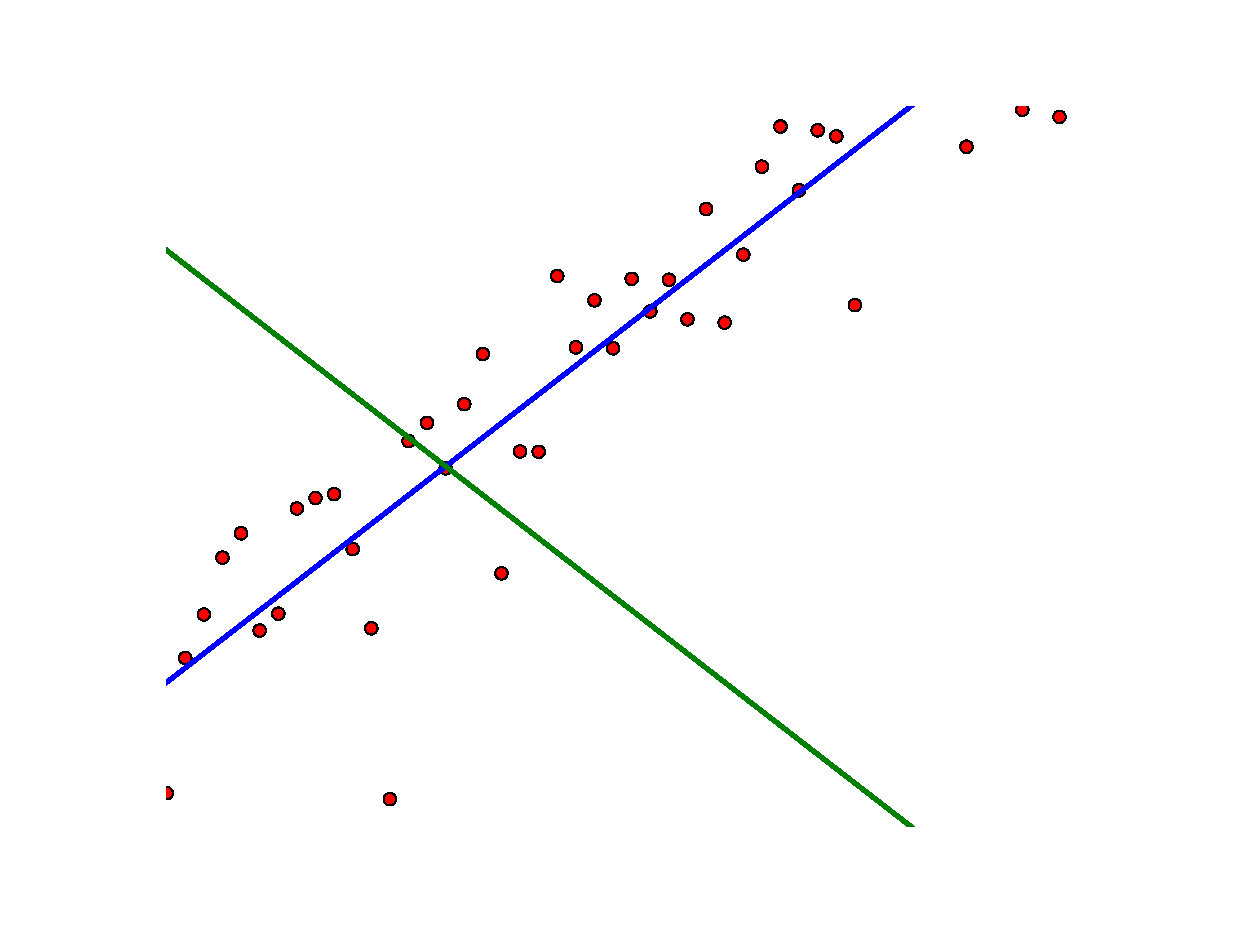
\includegraphics[height=6.5cm,width=7cm]{./figs/fig6.eps}
\caption{PCA:最大重构与最大可分}
\label{6}
\end{figure}

	\textbf{主成分分析(Principal Component Analysis,PCA)}:寻找一个超平面,使其具有两个很好的性质:\par
	\textbf{\textcircled{1}最大重构性}:样本点到这个超平面的距离足够近(近似误差小);\par
	\textbf{\textcircled{2}最大可分性}:样本点在超平面的投影尽可能分散(投影方差大)。\par
	对Fig6中的点,蓝色直线即是PCA所求的超平面,绿色直线是该超平面的正交。最大重构性表明点到蓝色直线的距离之和最近,即到绿色直线的正交投影之和最小;最大可分性表明点到蓝色直线的正交投影之和最大,即到绿色直线的距离之和最大。\par
	PCA的一种实现手段即是SVD,取出最大奇异值,它对应的维度容纳信息量最大,即是主成分。\par
	SVD作为线性代数理论的集大成者,有诸多应用:\par
	\textcircled{1}求矩阵的四个子空间;\par
	\textcircled{2}数值计算:判断方程是否有解,并求近似解(回归);\par
	\textcircled{3}压缩去噪:取少量较大奇异值,便可得到大部分信息;\par
	\textcircled{4}向量组的模式识别(Pattern Recognition):取最大奇异值;\par
	\textcircled{5}潜在语义索引(Latent Semantic Indexing,LSI):取较大奇异值,每个对应一种语义\par
	\textcircled{6}$\cdots\cdots$
	
	
	
	
\end{CJK}
\end{document}


